\clearpage
\chapter*{Preface}
\addcontentsline{toc}{chapter}
{Preface}
This report is written by students at the 4th semester of the education Maths-Technology at Aalborg University. The theme of the report is \textit{Signals and systems} and concerns time and frequency analysis of music signals. The premises for reading the report is knowledge of fundamental mathematical analysis. The developed scripts are written in the programming language Python 2.7, and all of the supplemental files can be downloaded through GitHub (see also appendix \ref{app:sup}): \url{https://github.com/TrineNyholm/G4-101a-P4/}.
\\ \\
The project group wishes to thank the supervisors Peter Koch from the Department of Electronic Systems and Henrik Garde from the Department of Mathematical Sciences for their confident, solid and helpful supervising throughout the project. Furthermore, the group wishes to thank the fellow group G4-101b for brewing morning coffee for four months.
\\ \\
Citations in the report are of the format [pages [number], citation], where the citation number refers to the bibliography. Book sources and web pages are specified with the information available, and web pages are furthermore noted with a visiting date. References to equations are written as numbers in parantheses only, and references to figures, chapters, sections, and so on are referred to as e.g. figure [number]. Only equations that are later referenced are numbered. Lastly, $j$ denotes the imaginary unit in this report, that is $j^2 = -1$.
\\ \\
\vspace{\baselineskip}\hfill Aalborg University, \today
\vfill\noindent

\begin{figure}[H]
\centering
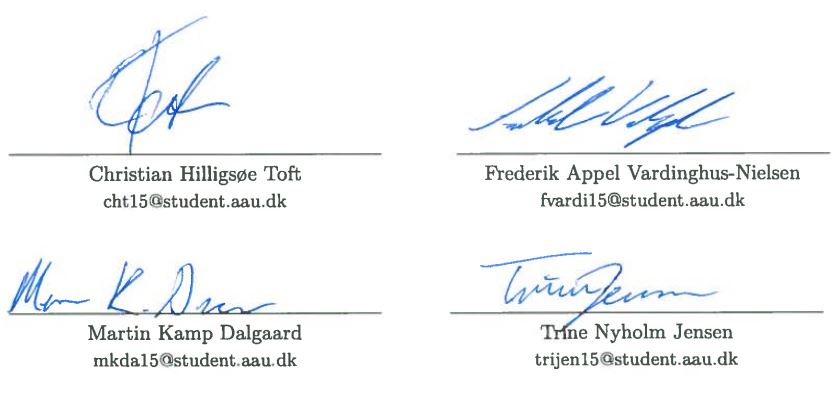
\includegraphics[width = \textwidth]{figures/preface.jpg}
\end{figure}